\documentclass[aspectratio=169,10pt]{beamer}

\usetheme[
  color=red,
  font=lato,
  titlefont=avantgarde,
  footerlogo=hust,
  bar=thin,
  titlepage=cover,
  sectionpage=panel,
  numbering=fraction,
  progressbar=on,
  framebg=on
]{HUST}
\input{hust-setup}

\usepackage{amsmath,amssymb}
\usepackage{booktabs,graphicx,tabularx}
\graphicspath{{figures/}{../../HUST-Beamer-Theme/assets/}}

\usetikzlibrary{positioning,fit,backgrounds,calc}
\tikzset{
  box/.style={rounded corners=1.5pt,align=center,inner sep=2pt,minimum height=.62cm,font=\scriptsize},
  frz/.style={box,draw=hustnavy,fill=hustnavy!8},
  mix/.style={box,draw=hustamber,fill=hustyellow!30,thick},
  trn/.style={box,draw=hustmain,fill=hustmain!18,thick},
  plain/.style={box,draw=none,fill=none},
  flow/.style={-{Latex[length=1.5mm]},thick,hustblack},
  gate/.style={-{Latex[length=1.5mm]},thick,hustmain},
  dict/.style={-{Latex[length=1.5mm]},thick,hustnavy},
  group/.style={rounded corners=3pt,draw=hustgray,dashed,inner sep=4pt},
  note/.style={font=\tiny,text=hustblack!80,align=center}
}
\newcommand{\refm}[1]{\textsuperscript{\tiny[#1]}}
\newcommand{\tblcap}[1]{\par\vspace{1mm}{\centering\scriptsize{\color{hustmain}Table:} #1\par}}
\newcommand{\nextq}[1]{\vfill\raggedright{\small\color{hustmain}\textbf{Next:} #1}}

% Cover only: let the title run across the slide instead of the theme's left column.
\makeatletter\def\hustp@coverTextW{0.92}\makeatother
\setbeamerfont{title}{size=\LARGE}
\title[WEMoE for NLP]{Merging 5 GLUE NLP task using\texorpdfstring{\\}{ }Weight-Ensembling Mixture of Experts}
\subtitle{Few-shot router training across five GLUE tasks}
\author[Group 1]{Group 1\texorpdfstring{\\[2pt]}{ }{\small Nguyễn Bá Anh -- 20261218M\\ Nguyễn Thị Nhã Linh -- 20261262M}\texorpdfstring{\\[2pt]}{ }{\small\textcolor{blue!55!black}{Instructor: Nguyễn Kiêm Hiếu}}}
\institute{}
\date{}
\hypersetup{pdfauthor={Nguyễn Bá Anh; Nguyễn Thị Nhã Linh; Instructor: Nguyễn Kiêm Hiếu}}

\begin{document}

\begin{frame}[plain]
  \titlepage
\end{frame}

%% ---------- PART 1: PROBLEM ----------
\begin{frame}{One model per task does not scale}
  \centering
  \begin{tikzpicture}
    \node[frz,minimum width=2.1cm] (b) at (0,0) {Pretrained\\ model};
    \foreach \y/\n/\s in {1.1/A/1, 0/B/2, -1.1/C/T}{
      \node[frz,minimum width=2.5cm] (m\n) at (4.2,\y) {Model for task $\s$};
      \draw[flow] (b.east) -- (m\n.west);
    }
    \node[plain] at (4.2,.56) {$\vdots$};
    \node[note,anchor=west] at (5.6,0) {\footnotesize one checkpoint per task};
  \end{tikzpicture}
  \vfill
  \raggedright
  \begin{itemize}
    \item \textbf{Management:} every new task adds another full model to train, store and serve.
    \item \textbf{Isolation:} each model knows only its own task, so nothing it learned is shared.
    \item \textbf{Redundancy:} the models start from the same weights, yet that common part is stored again each time.
  \end{itemize}
  \nextq{can these separate models become a single model?}
\end{frame}

\begin{frame}{Problem statement}
  \centering
  \begin{tikzpicture}
    \node[frz,minimum width=4.1cm,minimum height=1.25cm,font=\footnotesize] (i) at (0,0) {\textbf{Input}\\ pretrained weights $\theta_0$\\ task-specific weights $\theta_i,\ i\in\mathcal{T}$};
    \node[mix,minimum width=2.3cm,minimum height=1.25cm,font=\footnotesize] (c) at (4.3,0) {\textbf{Merge}\\ $\theta_{\mathrm{mer}}=C(\theta_0,\theta_i)$};
    \node[trn,minimum width=4.1cm,minimum height=1.25cm,font=\footnotesize] (o) at (8.6,0) {\textbf{Output}\\ one multi-task model:\\ (text, task) $\to$ label};
    \draw[flow] (i) -- (c);
    \draw[flow] (c) -- (o);
  \end{tikzpicture}
  \vfill
  \raggedright
  \textbf{Find the merge function $C$ so that the merged model:}
  \begin{itemize}
    \item integrates task knowledge \textbf{dynamically}, depending on the input;
    \item stays close to the quality of the task-specific models;
    \item needs fewer stored parameters than keeping all the models.
  \end{itemize}
  \nextq{why is a simple merge not enough?}
\end{frame}

\begin{frame}{Why this problem: static merging falls short}
  \begin{columns}[T]
    \begin{column}{.48\linewidth}
      \textbf{Why it is worth solving}
      \begin{itemize}
        \item Real systems serve many related NLP tasks.
        \item A shared model makes knowledge reusable across tasks.
        \item Merging needs no joint retraining from scratch.
      \end{itemize}
    \end{column}
    \begin{column}{.48\linewidth}
      \textbf{Why it is hard}
      \begin{itemize}
        \item \textbf{Interference:} updates from different tasks can conflict in the same parameters.
        \item \textbf{Sign disagreement:} models can pull one weight in opposite directions.
        \item \textbf{Static weights:} one fixed result cannot be the best for every task at once.
      \end{itemize}
    \end{column}
  \end{columns}
  \vfill
  \begin{block}{Gap}
    The merged weights should change with the input, not stay fixed for all inputs.
  \end{block}
  \nextq{how can weights depend on the input?}
\end{frame}

%% ---------- PART 2: IDEA ----------
\begin{frame}{Idea: Mixture of Experts}
  \begin{columns}[c]
    \begin{column}{.36\linewidth}
      \centering
      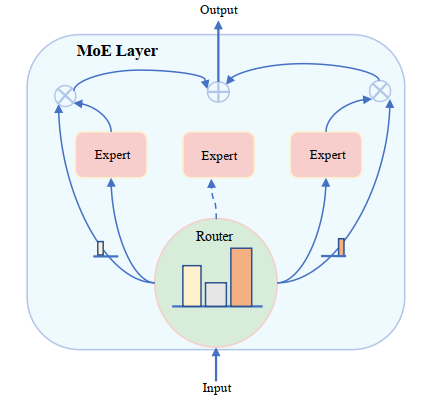
\includegraphics[height=3.7cm]{arch_moe}\\[-1mm]
      {\tiny Mixture of Experts layer\refm{6}}
    \end{column}
    \begin{column}{.62\linewidth}
      \[\mathrm{MoE}(x)=C\big(\{G_i(x)\cdot E_i(x)\}_{i=1}^{n}\big)\]
      \begin{itemize}
        \item Router $G$ decides how much each expert counts for \textbf{this input}.\refm{1}
        \item That is exactly the dynamic behaviour the problem asks for.
      \end{itemize}
    \end{column}
  \end{columns}
  \vfill
  \begin{block}{From outputs to weights}
    Running every expert is what we want to avoid. \textbf{WEMoE} mixes experts in \textbf{weight space}: the expert is a task vector, and one forward pass is enough.\refm{2}
  \end{block}
  \nextq{which backbone do we merge?}
\end{frame}

%% ---------- PART 3: THEORY ----------
\begin{frame}{BERT encoder: the shared backbone}
  \centering
  \begin{tikzpicture}[x=1cm,y=1cm]
    % full model
    \node[plain] (x) at (.75,0) {Tokens $x$: \texttt{[CLS]} $A$ \texttt{[SEP]}\\ (+ $B$ \texttt{[SEP]} for pairs)};
    \node[frz,minimum width=2.35cm] (emb) at (3.75,0) {Embeddings\\ token + segment + position\\ then LayerNorm};
    \node[frz,minimum width=2.3cm,very thick] (enc) at (6.75,0) {\textbf{Encoder layer} $\ell$\\ repeated $\times 12$};
    \node[frz,minimum width=1.75cm] (pool) at (9.2,0) {Pooler\\ {[CLS]}: dense, tanh};
    \node[frz,minimum width=1.6cm] (head) at (11.35,0) {Head $g_t$\\ dropout, linear};
    \node[plain] (out) at (13.1,0) {Logits\\ $\to\hat y$};
    \foreach \a/\b in {x/emb,emb/enc,enc/pool,pool/head,head/out} \draw[flow] (\a) -- (\b);
    % one encoder layer
    \node[plain] (in) at (.55,-1.75) {$h$};
    \node[frz,minimum width=1.9cm] (att) at (2.25,-1.75) {Multi-head\\ self-attention};
    \node[frz,minimum width=.95cm] (an1) at (4.2,-1.75) {Add\\ \&Norm};
    \node[mix,minimum width=1.2cm] (fc1) at (6.05,-1.75) {Linear\\ $W_1,b_1$};
    \node[frz,minimum width=.85cm] (act) at (7.5,-1.75) {GELU};
    \node[mix,minimum width=1.2cm] (fc2) at (8.95,-1.75) {Linear\\ $W_2,b_2$};
    \node[frz,minimum width=.95cm] (an2) at (10.85,-1.75) {Add\\ \&Norm};
    \node[plain] (outh) at (12.4,-1.75) {$h'$};
    \foreach \a/\b in {in/att,att/an1,an1/fc1,fc1/act,act/fc2,fc2/an2,an2/outh} \draw[flow] (\a) -- (\b);
    % residual connections
    \coordinate (r1) at ($(in.east)!.45!(att.west)$);
    \coordinate (r2) at ($(an1.east)!.45!(fc1.west)$);
    \draw[flow] (r1) -- ++(0,.62) -| (an1.north);
    \draw[flow] (r2) -- ++(0,.62) -| (an2.north);
    % groups
    \begin{scope}[on background layer]
      \node[group,draw=hustamber,thick,fit=(fc1)(act)(fc2)] (mlp) {};
      \coordinate (ltop) at ($(r1)+(0,.62)$);
      \coordinate (lbot) at ($(mlp.south)+(0,-.3)$);
      \node[group,inner sep=5pt,fit=(in)(outh)(att)(an2)(ltop)(lbot)] (lay) {};
    \end{scope}
    \draw[hustgray,dotted,thick] (enc.south west) -- (lay.north west);
    \draw[hustgray,dotted,thick] (enc.south east) -- (lay.north east);
    % labels
    \node[font=\scriptsize\bfseries,text=hustamber!85!black,anchor=north] at (mlp.south) {MLP block: its linear layers are upscaled later by WEMoE};
    \node[note,anchor=north west] at ([yshift=-1pt]lay.south west) {\scriptsize $h'=\mathrm{LayerNorm}\big(h+\mathrm{Sublayer}(h)\big)$};
    \node[note,anchor=north east] at ([yshift=-1pt]lay.south east) {\scriptsize $\mathrm{MLP}(h)=W_2\,\mathrm{GELU}(W_1h+b_1)+b_2$};
  \end{tikzpicture}
  \vfill
  \raggedright
  \begin{itemize}\footnotesize
    \item \texttt{bert-base-uncased}: 12 encoder layers, 109.5M parameters.\refm{3} All experts share this structure, so weights can be subtracted and added position by position.
    \item Self-attention gives each token a state that reflects its whole context. The {[CLS]} state passes through the pooler to the head of task $t$.
    \item CoLA and SST-2 use a single sentence; MRPC, RTE and QNLI use a sentence pair.
  \end{itemize}
  \nextq{how is this structure merged?}
\end{frame}

\begin{frame}{WEMoE architecture: two kinds of merging}
  \centering
  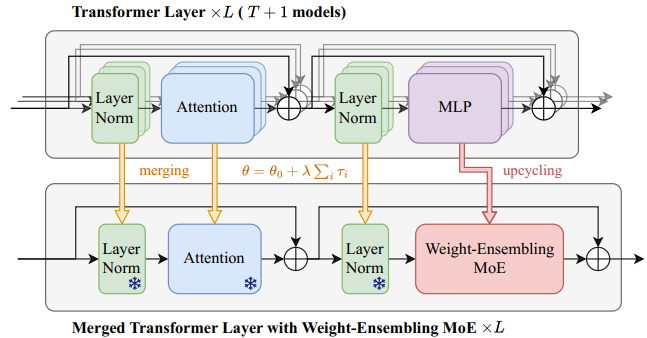
\includegraphics[height=3.35cm]{arch_wemoe_overview}\\[-.5mm]
  {\tiny Top: the fine-tuned and pretrained models. Bottom: the merged layer.\refm{2}}
  \vfill
  \raggedright
  \begin{itemize}\footnotesize
    \item \textbf{Static:} weights outside the MLP are merged once with Task Arithmetic. In this project that also covers embeddings and pooler.
    \item \textbf{Dynamic:} each MLP is upscaled to a Weight-Ensembling MoE module, so its weights depend on the input.
    \item Frozen parts carry the snowflake mark; only the router will be trained.
  \end{itemize}
  \nextq{first the static part, then the module.}
\end{frame}

\begin{frame}{Task Arithmetic: static merge with task vectors}
  \begin{columns}[c]
    \begin{column}{.3\linewidth}
      \centering
      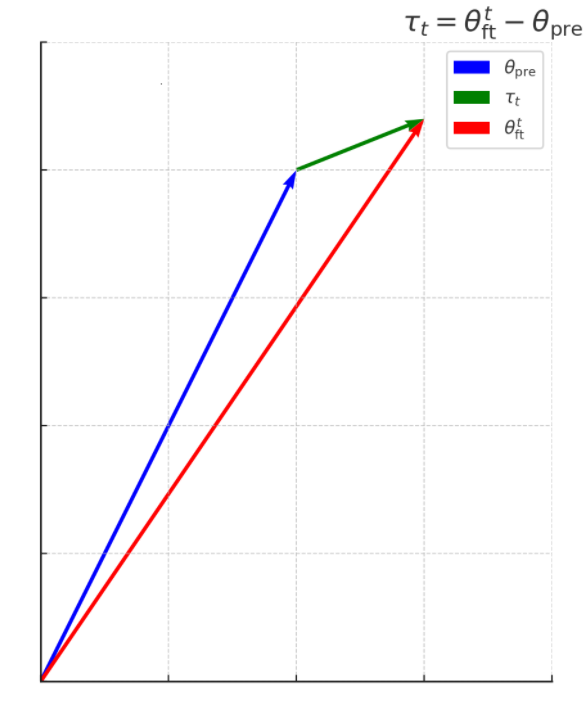
\includegraphics[height=3.6cm]{arch_task_vector}
    \end{column}
    \begin{column}{.68\linewidth}
      \textbf{Task vector:} what fine-tuning changed for task $i$\refm{4}
      \[\tau_i=\theta_i-\theta_0\qquad(\theta_{\mathrm{pre}}=\theta_0,\ \ \theta_{\mathrm{ft}}^{\,i}=\theta_i)\]
      \textbf{Task Arithmetic:} add the vectors back to the base
      \[\theta=\theta_0+\lambda\sum_{i=1}^{n}\tau_i\]
    \end{column}
  \end{columns}
  \vfill
  \begin{itemize}\footnotesize
    \item $\lambda$ controls how strongly the task vectors contribute; it is chosen on dev.
    \item Simple and compact, but the result is the same for every input.
  \end{itemize}
  \nextq{make the coefficients depend on the input, in the MLPs.}
\end{frame}

\begin{frame}{Router and WEMoE module: input-conditioned MLP}
  \begin{columns}[c]
    \begin{column}{.36\linewidth}
      \centering
      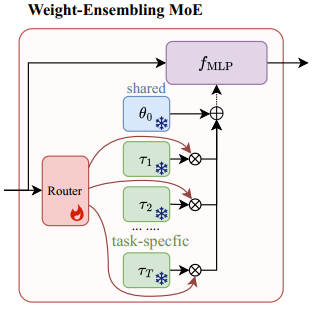
\includegraphics[height=3.7cm]{arch_wemoe_module}\\[-.5mm]
      {\tiny WEMoE module; here $T=5$\refm{2}}
    \end{column}
    \begin{column}{.62\linewidth}
      \[w^{\ell}(x)=\frac{1}{N}\sum_{j=1}^{N}r^{\ell}(h_j)\in\mathbb{R}^{5}\]
      \[W^{\ell}(x)=W_0^{\ell}+\sum_{e=1}^{5}w_e^{\ell}(x)\,\tau_e^{\ell}\]
      \[r^{\ell}(h)=\mathrm{fc}_2\big(\mathrm{ReLU}(\mathrm{fc}_1(h))\big)\]
    \end{column}
  \end{columns}
  \vfill
  \begin{itemize}\footnotesize
    \item One router per encoder layer; the mean runs over non-padding tokens; both MLP linear layers share $w^{\ell}$.
    \item No softmax: a weight can exceed 1 or be negative, so a router can amplify or subtract a task vector.
    \item The router's bias starts at $\lambda$, so the model starts close to Task Arithmetic.
  \end{itemize}
\end{frame}

\begin{frame}{Objective: few-shot fine-tuning (FSFT)}
  \textbf{Cross-entropy on a small labelled set, summed over the tasks:}
  \[
    \min_{\phi}\ \sum_{t=1}^{5}\ \frac{1}{|B_t|}\sum_{(x,y)\in B_t}-\log p_{\phi}(y\mid x,t),
    \qquad B_t\subset D_t^{(k)},\ \ |D_t^{(k)}|=k
  \]
  \begin{itemize}
    \item $\phi$: router parameters, \textbf{the only trainable weights} (7.1M).
    \item $D_t^{(k)}$: $k$ labelled examples of task $t$, which the experts have never seen.
    \item $p_{\phi}$: softmax over the logits of head $g_t$.
  \end{itemize}
  \vfill
  \centering
  \begin{tikzpicture}
    \node[frz,minimum width=2.9cm] (a) at (0,0) {$\tau_e$, $W_0$, non-MLP, heads\\ frozen};
    \node[trn,minimum width=2.4cm] (b) at (4,0) {Routers $\phi$\\ updated by gradient};
    \node[mix,minimum width=2.6cm] (c) at (8,0) {Best step\\ chosen on dev};
    \draw[flow] (a) -- (b);
    \draw[flow] (b) -- (c);
  \end{tikzpicture}
  \nextq{how does the whole pipeline run?}
\end{frame}

%% ---------- PART 4: EXPERIMENTS ----------
\begin{frame}{Implementation flow: from dataset to evaluation}
  \centering
  \begin{tikzpicture}[x=1cm,y=1cm,dat/.style={box,draw=hustgray,fill=white}]
    % stage panels
    \fill[hustnavy!4,rounded corners=3pt] (-.3,-2.65) rectangle (2.75,2.5);
    \fill[hustnavy!4,rounded corners=3pt] (3.1,-2.65) rectangle (6.2,2.5);
    \fill[hustyellow!12,rounded corners=3pt] (6.55,-2.65) rectangle (10.1,2.5);
    \fill[hustnavy!4,rounded corners=3pt] (10.45,-2.65) rectangle (13.75,2.5);
    \node[font=\scriptsize\bfseries,text=hustmain] at (1.22,2.25) {1. Dataset};
    \node[font=\scriptsize\bfseries,text=hustmain] at (4.65,2.25) {2. Fine-tune};
    \node[font=\scriptsize\bfseries,text=hustmain] at (8.33,2.25) {3. Train WEMoE};
    \node[font=\scriptsize\bfseries,text=hustmain] at (12.1,2.25) {4. Evaluate};
    % 1. dataset and its splits
    \node[dat,minimum width=2.75cm] (d) at (1.22,1.45) {\textbf{5 GLUE tasks}\\ MRPC, RTE, CoLA,\\ SST-2, QNLI};
    \node[dat,minimum width=2.2cm,minimum height=.5cm] (tr) at (1.5,.6) {Expert train};
    \node[dat,minimum width=2.2cm,minimum height=.5cm] (dv) at (1.5,-.35) {Dev};
    \node[dat,minimum width=2.2cm,minimum height=.5cm] (fs) at (1.5,-1.25) {Few-shot pool};
    \node[dat,minimum width=2.2cm,minimum height=.5cm] (va) at (1.5,-2.15) {Official validation};
    \draw[thick,hustblack] (.05,1.45 |- d.south) -- (.05,-2.15);
    \foreach \n in {tr,dv,fs,va}{\draw[flow] (.05,0 |- \n.west) -- (\n.west);}
    % 2. fine-tune
    \node[frz,minimum width=2.7cm] (p) at (4.65,1.5) {\textbf{Pretrained} $\theta_0$\\ \texttt{bert-base-uncased}};
    \node[frz,minimum width=2.7cm,minimum height=.9cm] (e) at (4.65,.6) {\textbf{Five experts} $\theta_i$, heads $g_i$\\ $\tau_i=\theta_i-\theta_0$};
    \draw[flow] (p) -- (e);
    \draw[flow] (tr.east) -- (e.west |- tr.east);
    % 3. train WEMoE
    \node[mix,minimum width=3.1cm,minimum height=1cm] (m) at (8.33,.6) {\textbf{Merge}\\ Outside MLP: Task Arithmetic\\ MLP: WEMoE modules};
    \node[trn,minimum width=3.1cm,minimum height=.9cm] (f) at (8.33,-1.25) {\textbf{FSFT: routers only}\\ $k$ examples per task\\ $\to$ one merged model};
    \draw[dict] (e.east) -- (m.west);
    \draw[flow] (9.3,0 |- m.south) -- (9.3,0 |- f.north);
    \draw[flow] (fs.east) -- (f.west);
    % dev selects in stages 2 and 3
    \draw[dict,dashed,-] (dv.east) -- (7.2,-.35);
    \draw[dict,dashed] (4.65,-.35) -- node[right,font=\tiny,text=hustnavy]{best epoch} (e.south);
    \draw[dict,dashed] (7.2,-.35) -- node[left,font=\tiny,text=hustnavy]{$\lambda$} (7.2,0 |- m.south);
    \draw[dict,dashed] (7.2,-.35) -- node[right,font=\tiny,text=hustnavy]{best step} (7.2,0 |- f.north);
    % 4. evaluate
    \node[frz,minimum width=3cm,minimum height=4.5cm,text width=2.8cm,align=left] (b) at (12.1,-.25) {\textbf{Reported on official validation only}\\[2mm] \textbf{Scores:} task score, average, gain over majority\\[2mm] \textbf{Compared with:} experts, Task Arithmetic, majority class\\[2mm] \textbf{Costs:} stored parameters, latency};
    \draw[flow] (f.east) -- (b.west |- f.east);
    \draw[flow] (va.east) -- (b.west |- va.east);
  \end{tikzpicture}
  \vfill
  \raggedright
  {\footnotesize Expert weights stay frozen after stage 2; only the routers learn in stage 3. The task id selects the head.}
\end{frame}

\begin{frame}{Data: five binary GLUE tasks}
  \centering
  \footnotesize
  \renewcommand{\arraystretch}{1.25}
  \begin{tabularx}{\linewidth}{>{\bfseries}l X l l l}
    \toprule
    Task & Decides whether\ldots & Input fields & Labels & Metric\\
    \midrule
    MRPC & two sentences are paraphrases & sentence1, sentence2 & not\_equivalent / equivalent & acc + F1\\
    RTE & a sentence entails another & sentence1, sentence2 & entailment / not\_entailment & accuracy\\
    CoLA & a sentence is grammatical & sentence & unacceptable / acceptable & MCC\\
    SST-2 & a sentence is positive or negative & sentence & negative / positive & accuracy\\
    QNLI & a sentence answers a question & question, sentence & entailment / not\_entailment & accuracy\\
    \bottomrule
  \end{tabularx}
  \vfill
  \raggedright
  \begin{itemize}
    \item GLUE benchmark.\refm{5} Inputs are tokenised to a maximum length of 128.
    \item \textbf{Task score:} MRPC uses the mean of accuracy and F1. Scores are $\times 100$.
    \item \textbf{Average score:} unweighted mean of the five task scores.
  \end{itemize}
\end{frame}

\begin{frame}{Data split: keep each stage's data apart}
  \centering
  \small
  \begin{tabular}{l r r r r r}
    \toprule
    Task & Official train & Few-shot pool & Dev & Expert train & Official validation\\
    \midrule
    MRPC & 3,668 & 256 & 367 & 3,045 & 408\\
    RTE & 2,490 & 256 & 249 & 1,985 & 277\\
    CoLA & 8,551 & 256 & 855 & 7,440 & 1,043\\
    SST-2 & 67,349 & 256 & 1,000 & 66,093 & 872\\
    QNLI & 104,743 & 256 & 1,000 & 103,487 & 5,463\\
    \midrule
    \textbf{Used for} & & \textbf{FSFT} & \textbf{Selection} & \textbf{Experts} & \textbf{Reporting}\\
    \bottomrule
  \end{tabular}
  \vfill
  \raggedright
  \begin{itemize}
    \item Official train is split once, with seed 42. Dev is 10\% of train, at most 1,000 examples.
    \item Experts never see the few-shot pool. $k$ examples per task are drawn from it.
    \item Every choice (expert epoch, $\lambda$, FSFT step) is made on dev. Official validation is used for reported scores only.
  \end{itemize}
\end{frame}

\begin{frame}{Stage 2: fine-tuning the five experts}
  \raggedright\small Hyperparameters:\par\vspace{1mm}
  \centering\footnotesize
  \renewcommand{\arraystretch}{1.3}\begin{tabular}{|l|c|c|c|c|c|}
    \hline
    \textbf{Setting} & \textbf{MRPC} & \textbf{RTE} & \textbf{CoLA} & \textbf{SST-2} & \textbf{QNLI}\\ \hline
    Learning rate & 2e-5 & 2e-5 & 2e-5 & 2e-5 & 2e-5\\ \hline
    Weight decay & 1e-2 & 1e-2 & 1e-2 & 1e-2 & 1e-2\\ \hline
    Scheduler type & linear & linear & linear & linear & linear\\ \hline
    Warmup ratio & 0.10 & 0.10 & 0.10 & 0.10 & 0.10\\ \hline
    Gradient clip norm & 1 & 1 & 1 & 1 & 1\\ \hline
    Batch size / epochs & 32 / 3 & 32 / 3 & 32 / 3 & 32 / 3 & 32 / 3\\ \hline
  \end{tabular}
  \tblcap{Fine-tuning settings of \texttt{bert-base-uncased}: one recipe for all five GLUE tasks.}
  \vfill
  \raggedright\small Results:\par\vspace{1mm}
  \centering\footnotesize
  \renewcommand{\arraystretch}{1.3}\begin{tabular}{|c|c|c|c|c|}
    \hline
    \textbf{MRPC (Acc/F1)} & \textbf{RTE (Acc)} & \textbf{CoLA (MCC)} & \textbf{SST-2 (Acc)} & \textbf{QNLI (Acc)}\\ \hline
    82.1 / 88.1 & 63.2 & 59.1 & 92.2 & 91.2\\ \hline
  \end{tabular}
  \tblcap{Expert scores on official validation ($\times 100$); average score 78.2. Best epoch on dev: 2, 3, 3, 2, 3.}
\end{frame}

\begin{frame}{Stage 3: merging and few-shot router training}
  \raggedright\small Hyperparameters:\par\vspace{.5mm}
  \centering\scriptsize
  \renewcommand{\arraystretch}{1.2}\begin{tabular}{|l|c|c|c|c|c|}
    \hline
    \textbf{Setting} & \textbf{Full, $k$=16} & \textbf{Full, $k$=64} & \textbf{Full, $k$=256} & \textbf{Intermediate, $k$=256} & \textbf{Input-indep., $k$=256}\\ \hline
    Upscaled MLP layers & both & both & both & first only & both\\ \hline
    Trainable parameters & 7.1M & 7.1M & 7.1M & 7.1M & 60\\ \hline
    Learning rate & 1e-4 & 1e-4 & 1e-4 & 1e-4 & 1e-3\\ \hline
  \end{tabular}
  \tblcap{All runs: AdamW, batch 16 per task, 500 steps, linear schedule, warmup 0.10, no weight decay, no gradient clipping. Task Arithmetic: $\lambda=0.3$, best on dev from $\{0.1,\dots,1.0\}$.}
  \vspace{1mm}
  \raggedright\small Results:\par\vspace{.5mm}
  \centering\scriptsize
  \renewcommand{\arraystretch}{1.25}\setlength{\tabcolsep}{4pt}\begin{tabular}{|l|c|c|c|c|c|c|}
    \hline
    \textbf{Metric} & \textbf{Task Arith.} & \textbf{Full, $k$=16} & \textbf{Full, $k$=64} & \textbf{Full, $k$=256} & \textbf{Interm., $k$=256} & \textbf{Input-indep., $k$=256}\\ \hline
    Average score & 57.4 & 60.8 $\pm$ 2.7 & 64.6 $\pm$ 3.7 & \textbf{69.9 $\pm$ 0.1} & 69.1 $\pm$ 0.1 & 58.4 $\pm$ 0.0\\ \hline
    Gain over majority & 18.4 & 25.5 & 46.7 & \textbf{59.1} & 54.8 & 20.0\\ \hline
    Best step of 500 & -- & 50, 0, 150 & 100, 250, 100 & 250, 200, 200 & 500, 400, 400 & 50, 50, 50\\ \hline
  \end{tabular}
  \tblcap{Official validation ($\times 100$), mean $\pm$ std over seeds 0, 1, 2 (a seed sets the router initialisation and the few-shot sample). Reference points: majority class 45.8, experts 78.2. Gain $=\frac{\text{score}-\text{majority}}{\text{expert}-\text{majority}}$, averaged over tasks.}
  \vfill
  \raggedright\footnotesize
  \textbf{Takeaway:} fixed coefficients barely move the score; input-conditioned routers close over half the gap. (Input-independent: one learning rate tried, dev score nearly flat.)
\end{frame}

\begin{frame}{Results by task: the gain is not uniform}
  \centering
  \footnotesize
  \renewcommand{\arraystretch}{1.3}\begin{tabular}{|l|c|c|c|c|c|}
    \hline
    \textbf{Model} & \textbf{MRPC (Acc/F1)} & \textbf{RTE (Acc)} & \textbf{CoLA (MCC)} & \textbf{SST-2 (Acc)} & \textbf{QNLI (Acc)}\\ \hline
    Majority class & 68.4 / 81.2 & 52.7 & 0.0 & 50.9 & 50.5\\ \hline
    Task Arithmetic & 68.6 / 81.3 & 47.3 & 16.9 & 69.8 & 77.9\\ \hline
    \textbf{WEMoE full, $k$=256} & 76.3$\pm$4.5 / 83.9$\pm$2.8 & \textbf{52.0 $\pm$ 4.4} & 42.6 $\pm$ 0.9 & 88.0 $\pm$ 0.5 & 86.7 $\pm$ 0.7\\ \hline
    WEMoE intermediate, $k$=256 & \textbf{66.5$\pm$0.7 / 76.6$\pm$1.0} & 59.0 $\pm$ 0.9 & 41.7 $\pm$ 0.9 & 86.7 $\pm$ 0.2 & 86.5 $\pm$ 0.2\\ \hline
    Single-task experts & 82.1 / 88.1 & 63.2 & 59.1 & 92.2 & 91.2\\ \hline
  \end{tabular}
  \tblcap{Per-task scores on official validation ($\times 100$), mean $\pm$ std over seeds 0, 1, 2.}
  \vfill
  \raggedright
  \begin{itemize}\footnotesize
    \item \textbf{Not solved everywhere:} full MLP does not reliably beat majority on RTE; intermediate-only falls below it on MRPC.
    \item \textbf{Budget matters:} small $k$ varies strongly across seeds (CoLA MCC std 14.1 at $k=16$, 17.8 at $k=64$); $k=256$ is stable on the average score.
  \end{itemize}
\end{frame}

\begin{frame}{Trade-offs and conclusion}
  \centering
  \footnotesize
  \renewcommand{\arraystretch}{1.3}\begin{tabular}{|l|c|c|c|c|}
    \hline
    \textbf{Deployment} & \textbf{Stored params} & \textbf{vs.\ 5 models} & \textbf{Avg score} & \textbf{ms/example (batch 32)}\\ \hline
    5 single-task models & 547.4M & 100.0\% & 78.2 & 1.61$^{*}$\\ \hline
    Task Arithmetic & 109.5M & 20.0\% & 57.4 & 1.63\\ \hline
    WEMoE, full MLP & 400.0M & 73.1\% & 69.9 & 7.31\\ \hline
    WEMoE, intermediate-only & 258.4M & 47.2\% & 69.1 & 4.69\\ \hline
  \end{tabular}
  \tblcap{Latency on one T4, random 128-token inputs, fp16. $^{*}$Times one expert: each input goes to its own expert by task id.}
  \vfill
  \raggedright
  \begin{itemize}\footnotesize
    \item \textbf{Answer:} input-conditioned merging with few-shot routers turns separate models into one, and clearly beats the static merge on average.
    \item \textbf{Cost:} it stays below the experts and is slower per example; the storage saving is largest for intermediate-only.
    \item \textbf{Limits:} RTE and MRPC remain weak; model selection uses more labels than FSFT trains on; experts use one seed; RTE and MRPC have small validation sets.
    \item This is one full run on five tasks, not a general guarantee.
  \end{itemize}
\end{frame}

%% ---------- BACKUP ----------

\begin{frame}{Backup: router details}
  \begin{itemize}
    \item Two linear layers with ReLU, applied per token; outputs are averaged over non-padding tokens.
    \item Initial weights are drawn with std 0.01 and the final bias is set to $\lambda$.
    \item Input-independent variant: one learned coefficient per expert per layer, 60 numbers in total.
    \item Experts do not run at inference: only the task vectors and heads are stored.
  \end{itemize}
\end{frame}

\begin{frame}{References}
  \footnotesize
  \begin{enumerate}
    \item[{[1]}] Shazeer et al. Outrageously Large Neural Networks: The Sparsely-Gated Mixture-of-Experts Layer. arXiv:1701.06538, 2017.
    \item[{[2]}] Tang et al. Merging Multi-Task Models via Weight-Ensembling Mixture of Experts. arXiv:2402.00433, 2024.
    \item[{[3]}] Devlin et al. BERT: Pre-training of Deep Bidirectional Transformers for Language Understanding. arXiv:1810.04805, 2019.
    \item[{[4]}] Ilharco et al. Editing Models with Task Arithmetic. arXiv:2212.04089, 2023.
    \item[{[5]}] Wang et al. GLUE: A Multi-Task Benchmark and Analysis Platform for Natural Language Understanding. arXiv:1804.07461, 2018.
    \item[{[6]}] Mu and Lin. A Comprehensive Survey of Mixture-of-Experts: Algorithms, Theory, and Applications. arXiv:2503.07137, 2025.
  \end{enumerate}
\end{frame}

\end{document}
